\chapter{Technology of ice reservoirs}
\label{chap:tech}

\cleanchapterquote{In building ice stupas, it's necessary to engage enough workforce to extract the water over
  long distances and to keep water flowing in cold temperatures.}{Marcus Nüsser}{(Professor, South Asia Institute)}

There is a long tradition of developing water harvesting structures in the upper Indus Basin, in both Ladakh,
northern India \citep{labbalTraditionalOasesLadakh2000, nusserIrrigationDevelopmentUpper2012} and various
locations in northern Pakistan \citep{kreutzmannScarcityOpulenceWater2011}. This is because land use in these
cold arid regions have always been prone to seasonal water scarcity, affecting irrigation and domestic water
supply \citep{dameSTONGDEREVISITEDLANDUSE2010, nusserLocalKnowledgeGlobal2016}. However, irrigated agriculture
continues to be a major, albeit declining, source of livelihood and food security in these regions
\cite{dameFoodSecurityHigh2011}. 

Due to the short growing period, central Ladakh is a single-cropping area with barley and wheat as important
staples, complemented by vegetables, pulses, and oil seeds. Depending on altitudinal position, irrigation with
complete flooding of fields (approximately 2-5 cm water column) starts between March and April prior to the
melting of high-altitude glaciers \citep{nusserSociohydrologyArtificialGlaciers2019}. Further, the unreliability
and the foreseen decrease of seasonal snow cover \citep{chevuturiClimateChangeLeh2018} increase the precariousness of the water
storage function of the cryosphere, especially in spring. In order to cope with recurrent water scarcity, many
water harvesting technologies and community arrangements have been developed
\citep{nusserSociohydrologyArtificialGlaciers2019} (see Fig. \ref{fig:AIRdesigns}). 

In this chapter, we focus on the ice terrace and ice stupa form of water harvesting technologies that are used
to conserve winter run-off water for utilization during summer. Through an analysis of their application in
Ladakh, we detail their construction process and cost. Then, we propose new strategies through which their
water loss, maintenance effort and cost can be reduced.

\begin{figure}[htb]
\centering
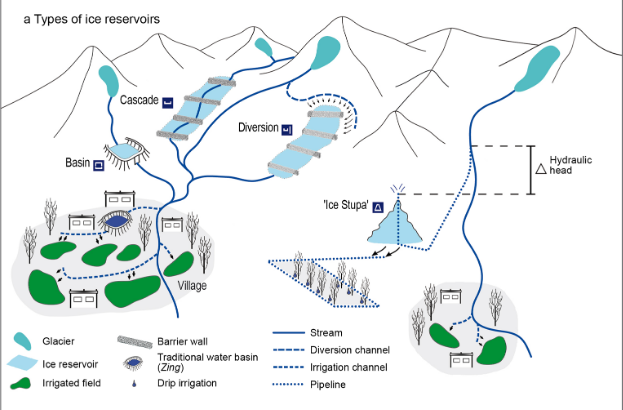
\includegraphics[width=12cm]{figs/AIR_designs.png}
\caption{Adapted from: \cite{nusserSociohydrologyArtificialGlaciers2019}}
\label{fig:AIRdesigns}
\end{figure}

\section{Ice terraces}

\begin{figure}[t]
\centering
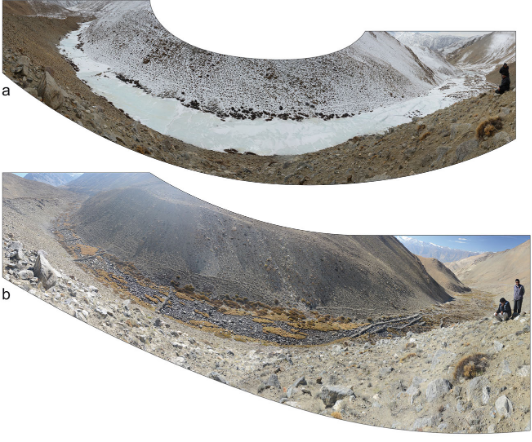
\includegraphics[width=12cm]{figs/IT_example.png}

\caption{Ice terrace of Phuktse, viewpoint 4430 m. (a) February 2014 (b) October 2014 Adapted from: \cite{nusserSociohydrologyArtificialGlaciers2019}}

\label{fig:ITexample}
\end{figure}

According to oral history and Corona imagery from 1969, the first ice terraces are older than 50 years and can
be found in Phuktse and Igoo. Over the past 30 years, 14 ice terraces have been constructed in central Ladakh,
located in tributary valleys of the Indus \citep{norphelArtificialGlacierHigh2009,
nusserSociohydrologyArtificialGlaciers2019}. Chewang Norphel, a well known engineer of the Leh Nutrition
Project, introduced this practice to Ladakh \citep{vinceGlacierMan2009}.  In February 2014, Phuktse built a
successful cascade with an almost continuous stretch of ice (Fig. \ref{fig:ITexample}). 

\subsection{Construction strategy}

There are two distinct types of ice terraces with site-specific modifications as shown in Fig.
\ref{fig:AIRdesigns}: the first type is built as cascades on perennial streams. A series of loose rock walls in
the river bed reduces flow velocity, but still lets water pass through. Such cascades allow flowing water to
freeze on exposed surfaces and form superimposed ice layers when temperatures drop (see Fig.
\ref{fig:ITscience}). 

The second type diverts water from streams with higher flow velocity to small side valleys, shaded by
surrounding mountains. This design allows to integrate higher slope positions for additional ice formation. It
consists of a series of partially cemented stone walls across the stream bed. Their dimensions are adjusted
based on the valley topography. The water for the ice terrace is obtained through a long diversion channel. 

\begin{figure}[htb]
\centering
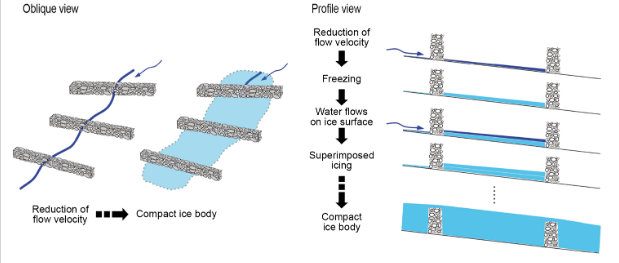
\includegraphics[width=12cm]{figs/IT_science.png}

\caption{ The process of ice accumulation for ice terraces Adapted from:
\cite{nusserSociohydrologyArtificialGlaciers2019}}

\label{fig:ITscience}
\end{figure}

As mentioned in the previous chapter, the design of the ice terraces is dependent on the suitability of the
site. Furthermore, the following construction guidelines are used depending on the terrain of the site
\cite{norphelSnowWaterHarvesting2015}:

\begin{itemize}

  \item If the section of the stream is very wide with a mild slope, then the stone walls are
    constructed in a series parallel to each other. The number and dimension of ice retaining walls depend on
    the flow of water available in the main stream during peak winter. In November, when winter begins, some
    locally available wild grass is put on the base of the dry bund to plug any holes.

  \item If the section of the stream is narrow with a steep grade then it needs to be diverted to a shady area
    by constructing a gravitational channel with a slope of 1:30. When it reaches the ice terrace site the slope
    should be gradually reduced to 1:50, allowing it to flow through small outlets to accelerate freezing. Stone
    walls need to be constructed parallel to the channel in series at a distance of 10-30 m, accoring to the
    natural slope of terrain. The steeper the terrain, the smaller the distance and slope between the bunds.

\end{itemize}


\subsection{Water storage and cost}

Ice volume variations of different ice terraces within Ladakh \citep{nusserSociohydrologyArtificialGlaciers2019,
norphelSnowWaterHarvesting2015} range from 510 $m^3$ to 81,040 $m^3$ highlighting the importance of local topography and
microclimate in their formation. The cost of construction depends on the size and number of stone walls
required. The estimated cost of ice terraces vary between 4600 to 15,330 USD
\cite{nusserSociohydrologyArtificialGlaciers2019}. The location requirements and the construction cost of ice
terraces, therefore, were prohibitive for widespread adoption.

\subsection{Improvement of construction tools}

% \begin{figure}[htb]
% \centering
% 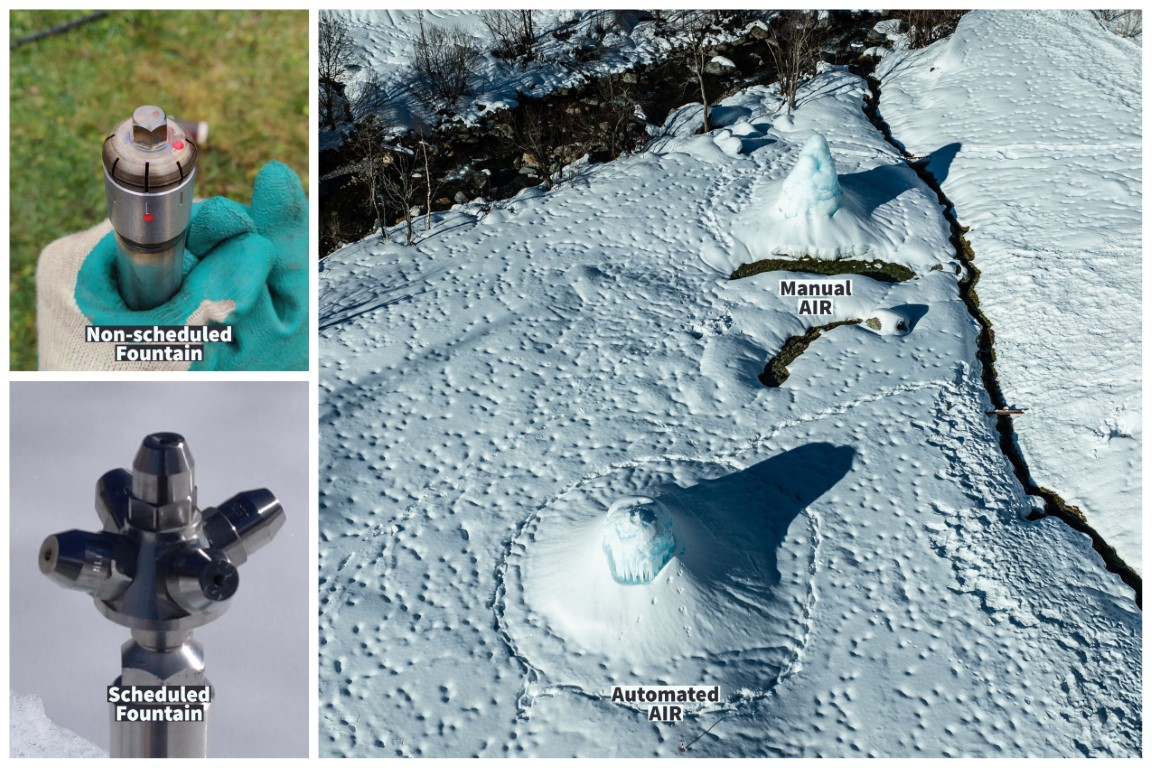
\includegraphics[width=12cm]{figs/AIR_fountains}
% \caption{Adapted from: \cite{nusserSociohydrologyArtificialGlaciers2019}}
% \label{fig:AIRdesigns}
% \end{figure}


\section{Ice stupas}

\begin{figure}[htb]
\centering
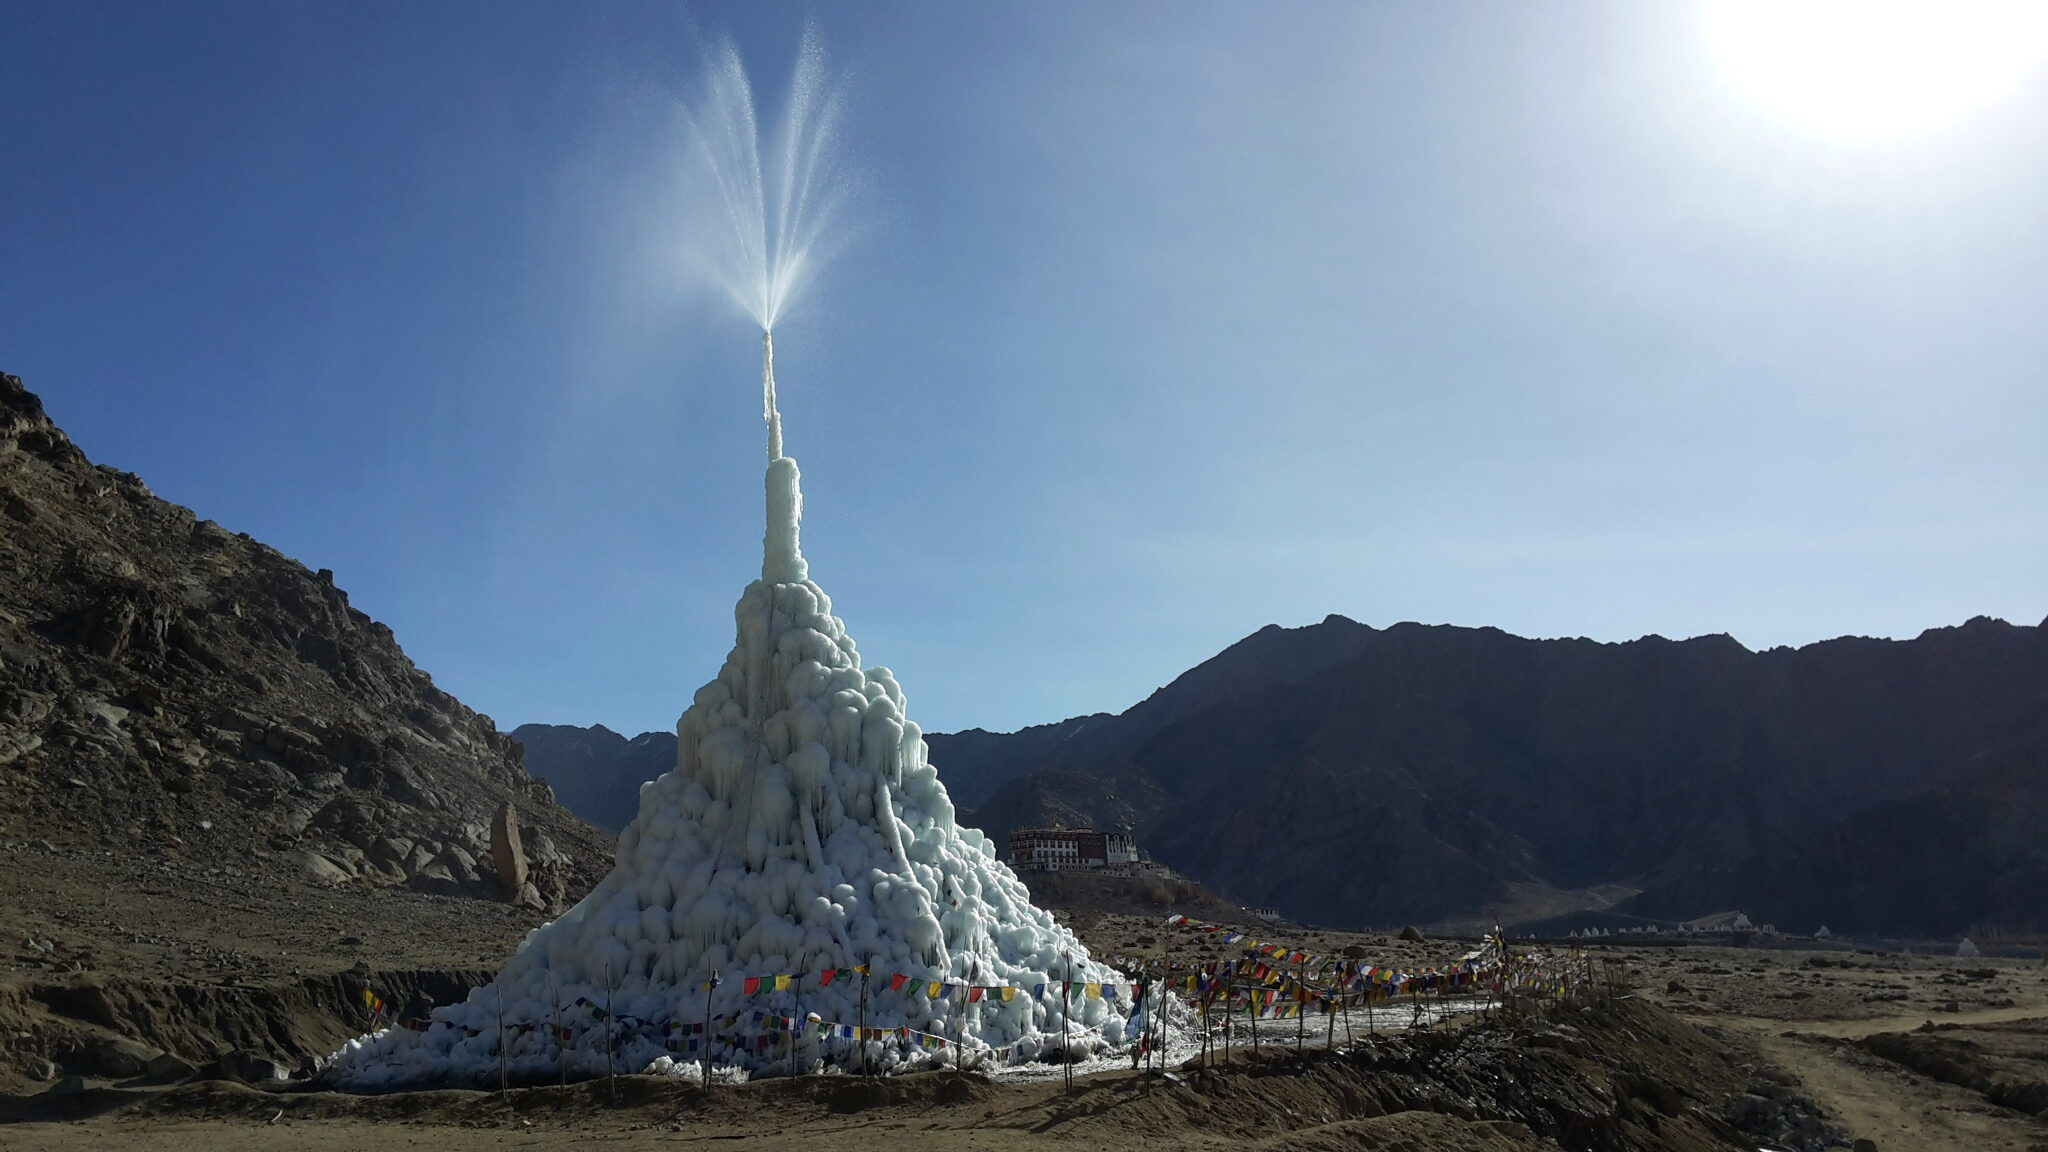
\includegraphics[width=12cm]{figs/IS_example.jpg}

\caption{Ice stupa of Shara}

\label{fig:ISexample}
\end{figure}

Ice stupas were invented by Sonam Wangchuk in 2013 \cite{wangchukIceStupaArtificial2014} to provide a much
cheaper alternative to achieve water storage compared to ice terraces. Ice stupas can also be placed much closer
to the plantations since they absorb lesser solar radiation per unit volume compared o ice terraces due to their
conical shape. However, the typical volume range of ice stupas (see Fig. \ref{fig:airs_ladakh}) are also much
smaller than ice terraces. Around 26 villages in Ladakh \cite{wangchukIceStupaCompetition2020} have integrated
ice stupas in their water resource management strategy.

\subsection{Construction strategy}

\begin{figure}[htb]
\centering
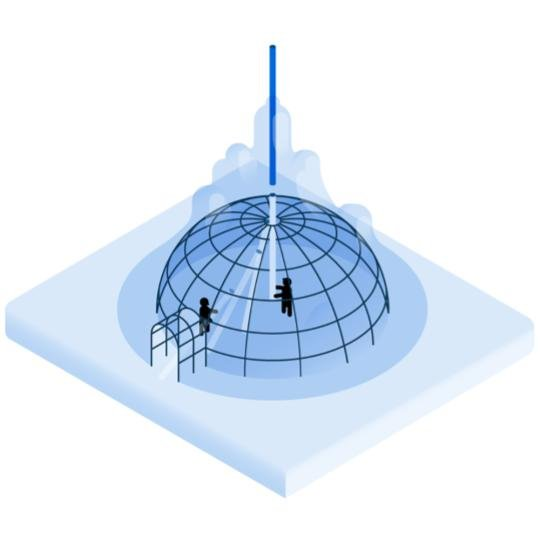
\includegraphics[width=8cm]{figs/IS_science.jpg}

\caption{The construction process of ice stupas. Diagrams by: Francesco Muzzi }

\label{fig:ISconstruction}
\end{figure}

A typical AIR (see Fig. \ref{fig:ISexample}) simply requires a fountain nozzle mounted on a supply pipeline. The
water source is usually a glacial stream. Due to the altitude difference between the pipeline input and fountain
output, water ejects from the fountain nozzle as droplets which freeze under subzero winter conditions. The
fountain is manually activated during winter nights. The fountain nozzle is raised through the addition of metal
pipes when significant ice accumulates below (see Fig. \ref{fig:ISconstruction}).  Typically, a dome of branches
is constructed around the metal pipes so that pipe extensions can be done from within this dome. Threads, tree
branches and fishing nets are used to guide and accelerate the ice formation.

\subsection{Water storage and cost}

\begin{figure}[htb]
\centering
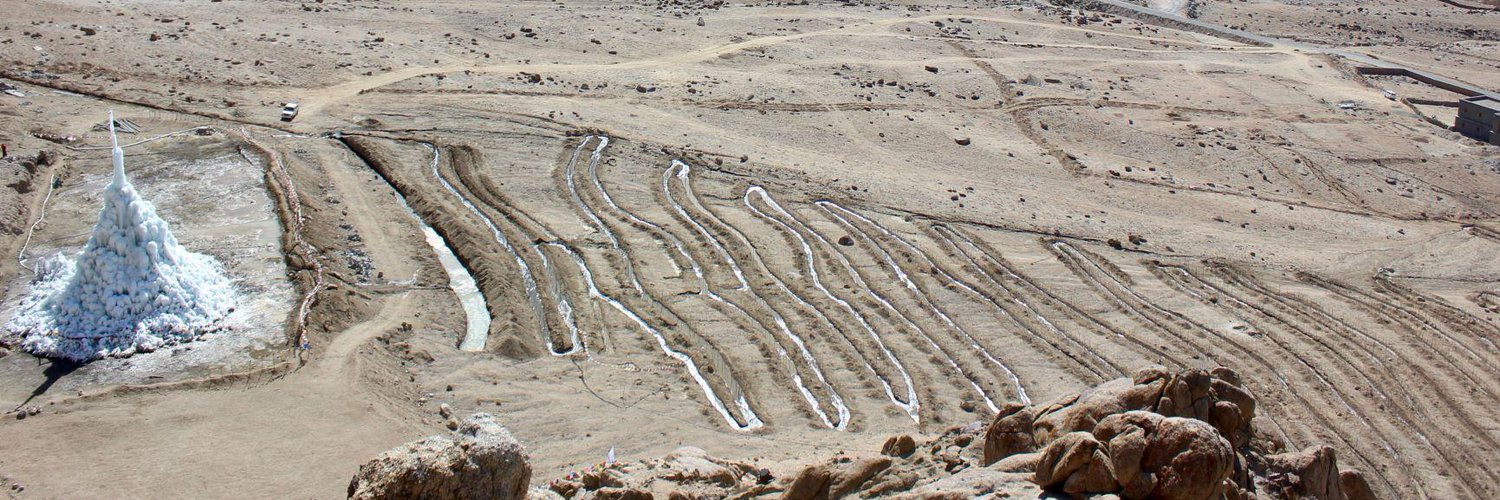
\includegraphics[width=12cm]{figs/IS_irrigation.jpeg}

\caption{Irrigation channel of the IN17 and IN18 AIRs. (P.C. Lobzang Dadul) }

\label{fig:ISirrigation}
\end{figure}

\begin{figure}[htb]
\centering
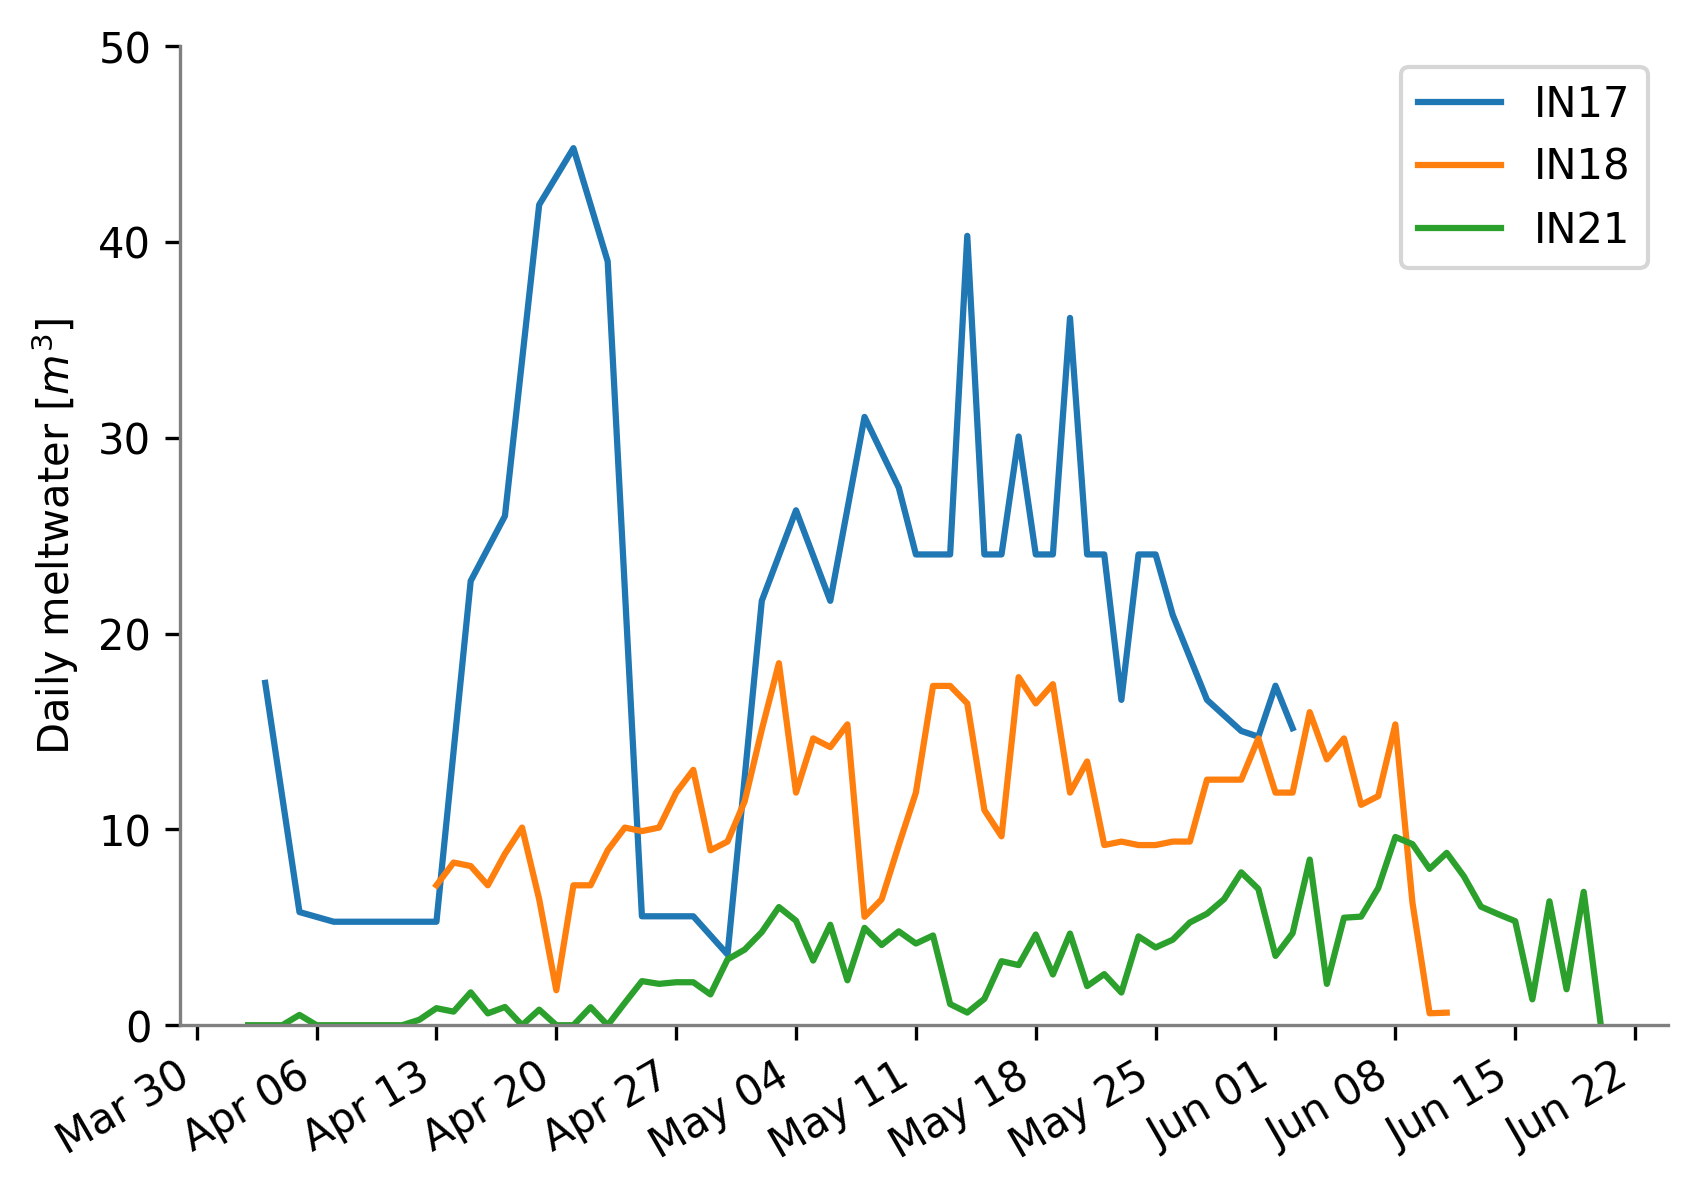
\includegraphics[width=12cm]{figs/melt.png}

\caption{Daily meltwater measurements for the IN17 and IN18 AIRs along with the corresponding model estimations
for the IN21 AIR. }

\label{fig:ISmelt}
\end{figure}

The cost of construction primarily depends on the material, size and length of the pipeline required. The
fountain nozzle cost is negligible in comparison. Typical pipeline configuration in Ladakh consists of a high
density polyethylene pipeline of 60 mm diameter and upto 5 km in length and 60 m of head. The estimated cost
of ice stupas vary between USD.

Fig. \ref{fig:ISmelt} shows the temporal variation of daily meltwater quantities obtained from 3 different AIRs
built in Ladakh during their melting periods (mid-April to mid-June). IN17 and IN18 AIRs were constructed in
Phyang village and their meltwater quantities was measured manually using the storage tank shown in Fig.
\ref{fig:ISirrigation}. The details of this measurement strategy are presented in Appendix. IN21 was constructed
in Gangles village and its meltwater quantities were modelled. The differences between the AIRs reflect the
corresponding interannual variability in the weather conditions. The average median daily AIR meltwater
quantities during these 3 melting seasons was around 12 million litres.    

\subsection{Suggested improvement of construction tools}

\subsubsection{Pipeline configuration}

The typical pipeline configuration in Ladakh is prone to pipeline freezing events. Therefore, the pipeline
material with higher insulation properties and diameter is required to lower this risk. Further effort is needed
to find a cost effective way to achieve an ideal pipeline configuration.

\subsubsection{Fountain nozzle}

Even though several AIR fountain nozzles exist, there does not exist a strategy to choose the best among them.
Their efficacy is expected to increase with lower droplet sizes, higher flight times and higher spray radius.
Therefore, a comparative study of all the AIR fountain nozzles used across these four factors would help make an
informed choice for future AIR constructions.

\subsubsection{Water supply management}

All the studied AIRs suffer from overwatering (paper I). Automated fountain water supply management has been
shown to increase their water use efficiency of AIRs and reduce their maintenance without compromising on their
meltwater production. The methodology to implement this new construction strategy is presented in paper II.


\section{Discussion}

\subsection{Ice terraces vs ice stupas}

\subsection{Artificial glaciers: A thought experiment}

% AIRs are a natural evolution of Ladakh's agricultural system. They can be related to traditional water
% harvesting technologies like the \textit{zing}, which are small tanks where meltwater is collected through the use
% of an intricate network of channels. The mountain oases of the Hindu Kush and Karakoram ranges
% have similar irrigation networks \citep{nusserLocalKnowledgeGlobal2016}.



% \begin{table}[h]
% 	\begin{tabularx}{\textwidth}{X | X | X}
% 		\hline
%     \textbf{Need} & \textbf{Daily meltwater requirement}& \textbf{Duration (days)} \\ \hline 
% 		Plantation irrigation			& 2 mm per m2				     & 2 months				\\
% 		Drinking water supply			& 1000 litres per person & 5				\\ 
% 		\hline
% 	\end{tabularx}
% 	\label{tab:table1}
% 	\caption{This is a caption text.}
% \end{table}

% \begin{table}[h]
% 	\begin{tabularx}{\textwidth}{X | X | X | X}
% 		\hline
%     \textbf{Technology}& \textbf{Water storage}& \textbf{Daily meltwater supply (days)}& \textbf{Duration} \\
%     \hline
% 		Ice terraces			& < 30				     & 2 months				\\ 
%     Ice stupas        & < 10             & 5				\\
% 		\hline
% 	\end{tabularx}
% 	\label{tab:table1}
% 	\caption{This is a caption text.}
% \end{table}

% Ice terraces are the oldest form of AIRs \citep{norphelArtificialGlacierHigh2009}. Usually situated below the
% glaciers at elevations where snowmelt starts end of March, these structures facilitate the freezing of stream
% water during winter at selected sites, usually shaded by surrounding mountains. 
